% !TEX root = ../main.tex

\chapter{Experiments}
\label{ch:experiments}

\section{Research Questions}
\begin{enumerate}
  \item Model analysis
  \item Bias
\end{enumerate}

\section{Experiments}
To analyze and compare the different models, I conducted the following experiments:
\begin{enumerate}
  \item Similar to \citet{oller_analyzing_2020}, I used RWG to draw the weights of the models and tested the performance on a Classic Control environment from OpenAI Gym.
  \item Second experiment
\end{enumerate}

In the first experiment, analogous to \citet{oller_analyzing_2020}, there is no learning involved. For their paper, they were interested in the complexity of the environment, whereas I aim to find out more about the nature of the models. I selected a few candidates for the models, which are described in Section~\ref{ssec:models} and used them for a series of experiments. First, I initialized the environment. I used the \verb|CartPole| and \verb|Acrobot| environment for these experiments. These environments are fairly easy to solve, as explained in Section~\ref{ssec:benchmarks}. Therefore, we expect some controllers to solve the task even without any training. Second, I initialized the respective model. Then, I drew the model weights from the standard normal distribution $\mathcal{N}(0,1)$. Each of these instances of the model represents a sample. In total, I used $10'000$ samples ($N_{samples}$). Finally, I ran 20 episodes ($N_{episodes}$) with each sample for an environment and stored the respective score as an entry of the score tensor $S$. Algorithm~\ref{alg:model-evaluation} shows an overview of the described procedure.
\begin{algorithm}
\caption{First experiment with RWG}
\begin{algorithmic}[1]
\State Initialize environment
\State Initialize model
\State Create array $S$ of size $N_{samples} \times N_{episodes}$
\For{$n = 1,2,...,N_{samples}$}
    \State Sample model weights randomly from $\mathcal{N}(0,1)$
    \For{$e=1,2,...,N_{episodes}$}
      \State Reset the environment
      \State Run episode with model
      \State Store accured episode reward in $S_{n,e}$
    \EndFor
\EndFor
\end{algorithmic}
\label{alg:model-evaluation}
\end{algorithm}

\subsection{OpenAI Gym Environments}
\begin{itemize}
  \item CartPole
  \item Acrobot
\end{itemize}

\subsection{Models}
\label{ssec:models}
To conduct the experiments, I used the following models: Neural Network models, Polynomial models.

For the polynomial model, I used two architectures. The first model $P_1$ consists of one polynomial for each possible action in the action space. The dimension of the weight vectors is according to the dimension of the input vector (observation). For the environment \verb|CartPole| with the discrete action space $\{0, 1\}$ and observation $x = [x_1, x_2, x_3, x_4]^T$, this means that $P_1$ consists of two polynomials:
\[
  p_0 = w_0^T x^3 + w_1^T x^2 + w_2^T x + w_3^T \mathbb{1} \in \mathbb{R}, \ \ \ \ \ x, w_i, \mathbb{1} \in \mathbb{R}^4
\]
\[
  p_1 = w_4^T x^3 + w_5^T x^2 + w_6^T x + w_7^T \mathbb{1} \in \mathbb{R}, \ \ \ \ \ x, w_i, \mathbb{1} \in \mathbb{R}^4
\]
The output of the model is decided according to the highest number. For \verb|CartPole|, this means:
\[
  P_1(x) =
  \begin{cases}1~&{\text{ if }}~p_0>p_1~,\\0~&{\text{ if }}~p_0<p_1~.\end{cases}
\]

The second model $P_2$ consists only of one polynomial. The output of the model is determined by a fixed threshold:
\[
  P_2(x) =
  \begin{cases}1~&{\text{ if }}~p_0<0.5~,\\0~&{\text{ if }}~p_0>0.5~.\end{cases}
\]
The output of the model has no reasonable upper and lower limit, as illustrated in Figure~\ref{fig:bounds}. To scale the output between 0 and 1, I used the logistic sigmoid function:
\begin{figure}[ht]
\centering
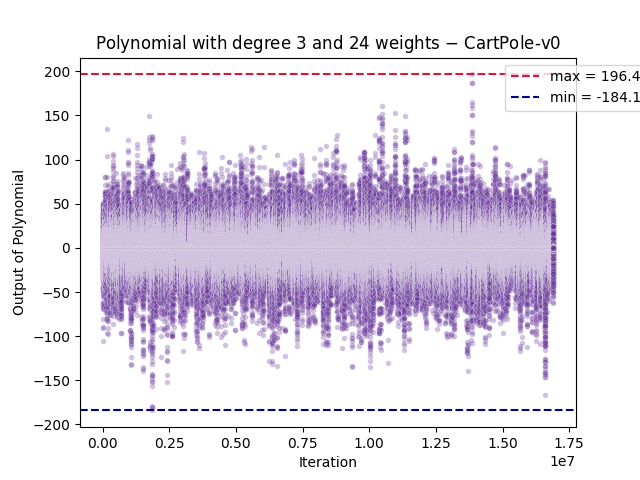
\includegraphics[width=0.7\textwidth]{PolynomialNN_degree_3_bounds}
\caption[Upper and lower bound]{
  \textbf{Upper and lower bound.}
  x
}
\label{fig:bounds}
\end{figure}
\[
  sig(x) = \frac{1}{1 + exp(-x)}
\]
The function $sig(x)$ has the typical S shape of a sigmoid function. A plot of the function is shown in Figure~\ref{fig:sigmoid}.

\begin{figure}[ht]
\centering
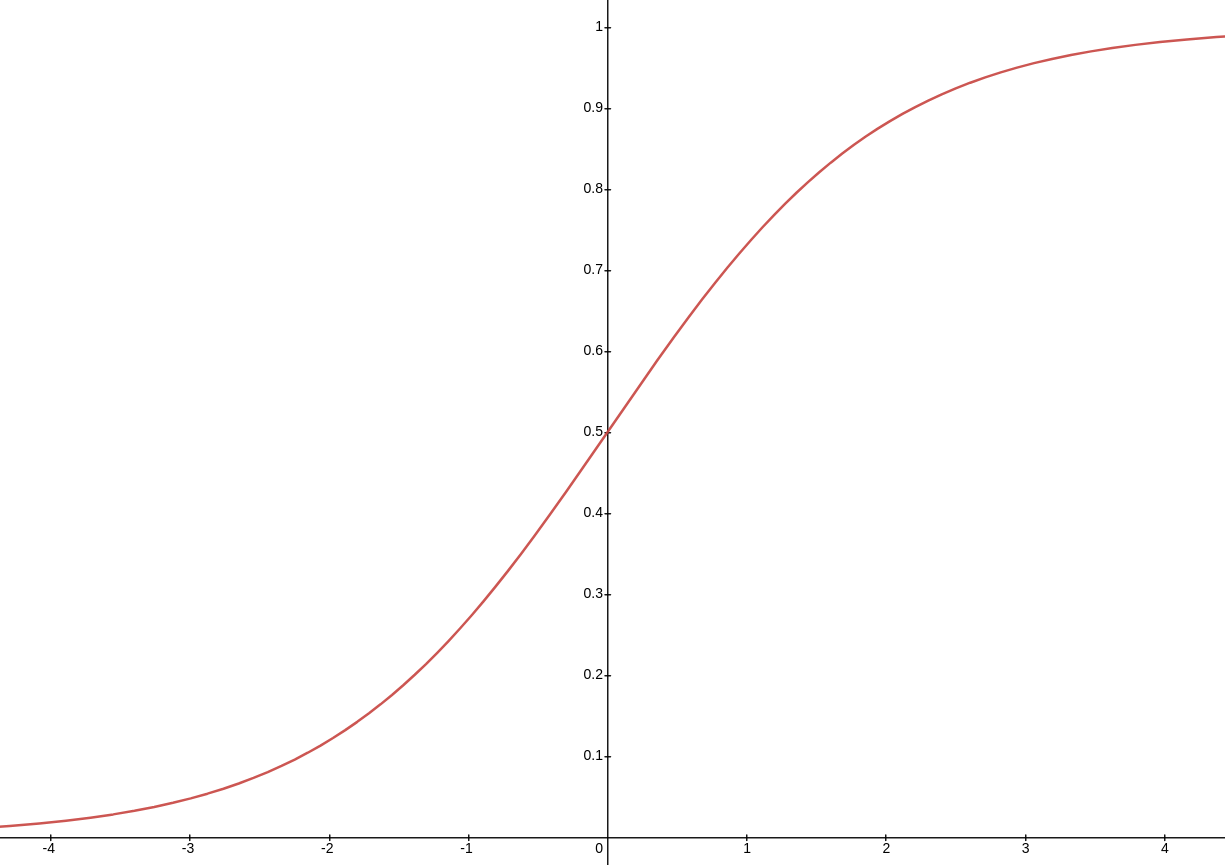
\includegraphics[width=0.5\textwidth]{sigmoid_small}
\caption[Simoid function]{
  \textbf{Sigmoid function.}
  The figures shows the plot of the logistic sigmoid function.
}
\label{fig:sigmoid}
\end{figure}

\begin{table}[h!] % positioning: here, enforced
\label{tab:example}
\center
\begin{tabular}{m{40mm}lllll}
  \toprule
  & bias & \# weights \\
  \midrule
  $Pol_1$ with bias & True & x \\
  $Pol_1$ without bias & False & x \\
  $Pol_2$ with bias & True & x \\
  $Pol_2$ without bias & False & x \\
  \bottomrule
  \end{tabular}
  \caption[Example]{%
    \textbf{Polynomial.}
    Description of structure of polynomial models.
  }
\end{table}


\section{Results}
\subsection{Experiment 1}
\begin{figure}[ht]
\centering
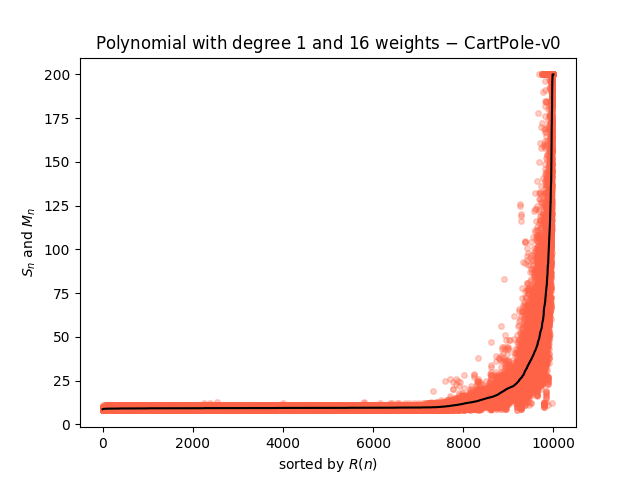
\includegraphics[width=0.329\textwidth]{experiment_1/PolynomialNN_degree_1_scatter_score}
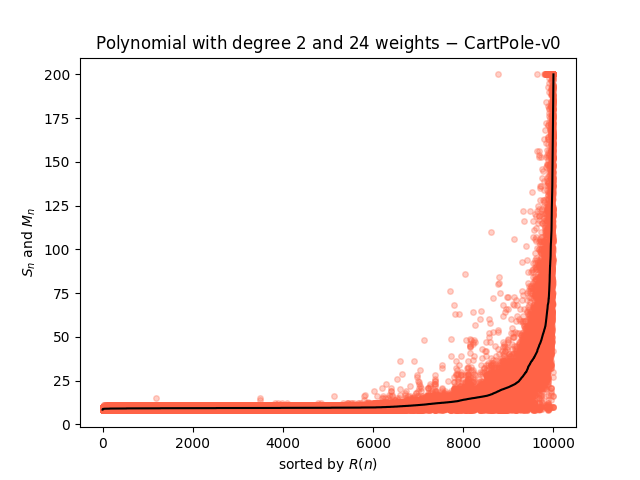
\includegraphics[width=0.329\textwidth]{experiment_1/PolynomialNN_degree_2_scatter_score}
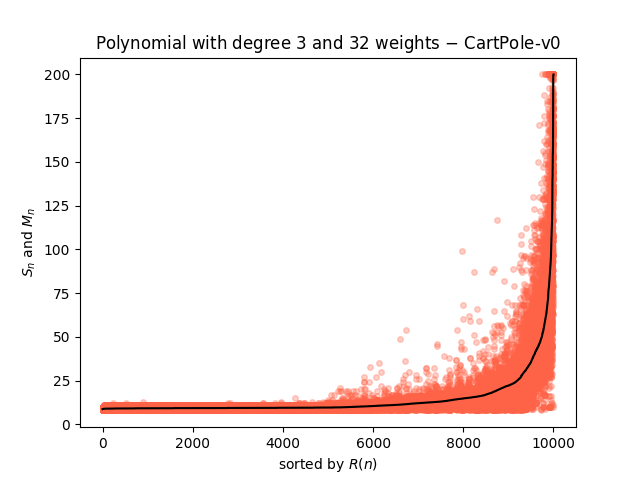
\includegraphics[width=0.329\textwidth]{experiment_1/PolynomialNN_degree_3_scatter_score}
\caption[Experiment 1: Polynomial]{
  \textbf{Polynomial.}
  x
}
\label{fig:polynomialNN_results}
\end{figure}


\subsubsection{Neural Network}

\subsubsection{Polynomial}

\section{Results}
